\documentclass[border=0.2cm, convert={density=600}]{standalone}
 
% Required packages and libraries
\usepackage{tikz}
\usetikzlibrary{shapes, positioning, arrows.meta}

% custom styles
\tikzset{
  parser/.style={
    rectangle,
    rounded corners,
    draw=black, very thick,
    minimum height=2em,
    inner sep=2pt,
    text centered,
    rectangle split,
    rectangle split draw splits=false,
    rectangle split parts=2,
    draw=black
  },
  arrow/.style={
    draw=black,
    thick,
    ->,
    >=stealth
  }
}

% custom dot symbol (bigger than \cdot but smaller than \bullet)
\makeatletter
\newcommand*\dotp{\mathpalette\dotp@{.5}}
\newcommand*\dotp@[2]{\mathbin{\vcenter{\hbox{\scalebox{#2}{$\m@th#1\bullet$}}}}}
\makeatother
 
\begin{document}
 
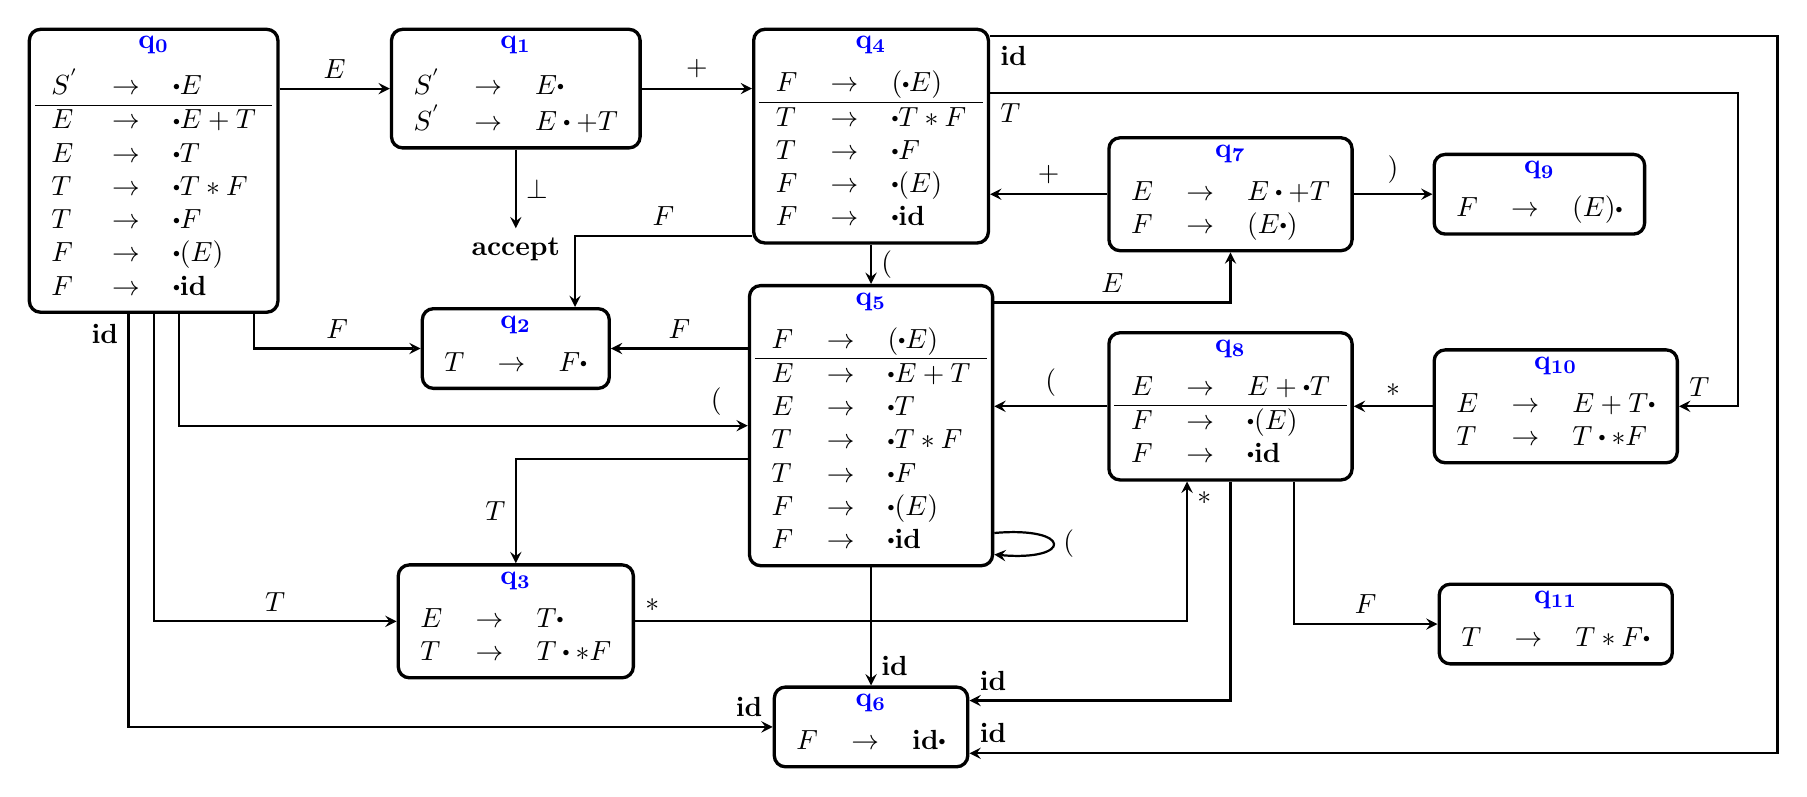
\begin{tikzpicture}
% nodes
\node[parser] (q0)
{ $\mathbf{\color{blue} q_{0}}$
  \nodepart{second}
  \begin{tabular}{lll}
    $S^{'}$ & $\rightarrow$ & $\dotp E$\\
    \hline
    $E$    & $\rightarrow$ & $\dotp E + T$\\
    $E$    & $\rightarrow$ & $\dotp T$\\
    $T$    & $\rightarrow$ & $\dotp T \ast F$\\
    $T$    & $\rightarrow$ & $\dotp F$\\
    $F$    & $\rightarrow$ & $\dotp (E)$\\
    $F$    & $\rightarrow$ & $\dotp \textbf{id}$\\
  \end{tabular}
};

\node[parser,
      right = 3cm of q0.north,
      anchor=north west] (q1)
{ $\mathbf{\color{blue} q_{1}}$
  \nodepart{second}
  \begin{tabular}{lll}
    $S^{'}$ & $\rightarrow$ & $E\dotp$\\
    $S^{'}$ & $\rightarrow$ & $E\dotp + T$
  \end{tabular}
};

\node[parser, below = 2cm of q1.south] (q2)
{ $\mathbf{\color{blue} q_{2}}$
  \nodepart{second}
  \begin{tabular}{lll}
    $T$ & $\rightarrow$ & $F\dotp$
  \end{tabular}
};

\node[parser, below = 2.2cm of q2.south] (q3)
{ $\mathbf{\color{blue} q_{3}}$
  \nodepart{second}
  \begin{tabular}{lll}
    $E$ & $\rightarrow$ & $T\dotp$\\
    $T$ & $\rightarrow$ & $T\dotp \ast F$
  \end{tabular}
};

\node[parser, right = 3cm of q1.north, anchor=north west] (q4)
{ $\mathbf{\color{blue} q_{4}}$
  \nodepart{second}
  \begin{tabular}{lll}
    $F$ & $\rightarrow$ & $(\dotp E)$\\
    \hline
    $T$ & $\rightarrow$ & $\dotp T \ast F$\\
    $T$ & $\rightarrow$ & $\dotp F$\\
    $F$ & $\rightarrow$ & $\dotp (E)$\\
    $F$ & $\rightarrow$ & $\dotp \textbf{id}$\\
  \end{tabular}
};

\node[parser, below = 0.5cm of q4.south] (q5)
{ $\mathbf{\color{blue} q_{5}}$
  \nodepart{second}
  \begin{tabular}{lll}
    $F$ & $\rightarrow$ & $(\dotp E)$\\
    \hline
    $E$     & $\rightarrow$ & $\dotp E + T$\\
    $E$     & $\rightarrow$ & $\dotp T$\\
    $T$     & $\rightarrow$ & $\dotp T \ast F$\\
    $T$     & $\rightarrow$ & $\dotp F$\\
    $F$     & $\rightarrow$ & $\dotp (E)$\\
    $F$     & $\rightarrow$ & $\dotp \textbf{id}$\\
  \end{tabular}
};

\node[parser, below = 1.5cm of q5.south] (q6)
{ $\mathbf{\color{blue} q_{6}}$
  \nodepart{second}
  \begin{tabular}{lll}
    $F$ & $\rightarrow$ & $\textbf{id}\dotp$
  \end{tabular}
};

\node[parser, right = 3cm of q4.center, anchor=north west] (q7)
{ $\mathbf{\color{blue} q_{7}}$
  \nodepart{second}
  \begin{tabular}{lll}
    $E$ & $\rightarrow$ & $E \dotp + T$\\
    $F$ & $\rightarrow$ & $(E \dotp)$
  \end{tabular}
};

\node[parser, below = of q7] (q8)
{ $\mathbf{\color{blue} q_{8}}$
  \nodepart{second}
  \begin{tabular}{lll}
    $E$ & $\rightarrow$ & $E + \dotp T$\\
    \hline
    $F$     & $\rightarrow$ & $\dotp (E)$\\
    $F$     & $\rightarrow$ & $\dotp \textbf{id}$\\
  \end{tabular}
};

\node[parser, right = of q7] (q9)
{ $\mathbf{\color{blue} q_{9}}$
  \nodepart{second}
  	\begin{tabular}{lll}
  		$F$ & $\rightarrow$ & $(E)\dotp$
  	\end{tabular}
};

\node[parser, right = of q8] (q10)
{ $\mathbf{\color{blue} q_{10}}$
  \nodepart{second}
  \begin{tabular}{lll}
    $E$ & $\rightarrow$ & $E + T \dotp$\\
    $T$ & $\rightarrow$ & $T \dotp \ast F$
  \end{tabular}
};

\node[parser, below = 1.5cm of q10] (q11)
{ $\mathbf{\color{blue} q_{11}}$
  \nodepart{second}
  \begin{tabular}{lll}
    $T$ & $\rightarrow$ & $T \ast F \dotp$
  \end{tabular}
};

\node[below = 1cm of q1] (ACC) {\textbf{accept}};

% edges
%% q0
\draw [arrow] (q1.center -| q0.east) -- node[anchor=south]{$E$}(q1.west);
\draw [arrow] (q0.south) -- (q0.south |- q3.west) -- node[anchor=south]{$T$} (q3.west);
\draw [arrow] (q0.-55) -- (q0.-55 |- q2.west) -- node[anchor=south]{$F$} (q2.west);
\draw [arrow] (q0.-80) |- (q5.west) node[anchor=south east,xshift=-2mm]{$($};
\draw [arrow] (q0.-100) node[anchor=north east]{\textbf{id}} |- (q6.west) node[anchor=south east]{\textbf{id}};

%% q1
\draw [arrow] (q1.south) -- node[anchor=west]{$\bot$} (ACC);
\draw [arrow] (q1.east) -- node[anchor=south]{$+$} (q1.east -| q4.west);

%% q3
\draw [arrow] (q3.east) node[anchor=south west]{$\ast$} -| (q8.-120) node[anchor=north west]{$\ast$};

%% q4
\draw [arrow] (q4.-140) -- node[anchor=south]{$F$} (q4.-140 -| q2.35) -- (q2.35);
\draw [arrow] (q4.south) -- node[anchor=west]{$($} (q5.north);
\draw [arrow](q4.40) node[anchor=north west]{\textbf{id}} -- ++(10cm,0) |- (q6.-15) node[anchor=south west]{\textbf{id}};
\draw [arrow](q4.20) node[anchor=north west]{$T$} -- ++(9.5cm,0) |- (q10.east) node[anchor=south west]{$T$};

%% q5
\draw [arrow] (q5.south) -- (q6.north) node[anchor=south west]{\textbf{id}};
\draw [arrow] (q5.195) -- (q5.195 -| q3.north) -- node[anchor=east]{$T$} (q3.north);
\draw [arrow] (q2.east -| q5.west) -- node[anchor=south]{$F$} (q2.east);
\draw [arrow] (q5.45) -- node[anchor=south]{$E$} (q5.45 -| q7.south) -- (q7.south);
\path [arrow, every loop/.style={min distance=10mm,out=5,in=-5,looseness=4}] (q5) edge[loop right, transform canvas={yshift=-15mm}] node[anchor=west]{$($} ();

%% q7
\draw [arrow] (q7.east) -- node[anchor=south]{$)$} (q9.west);
\draw [arrow] (q7.west) -- node[anchor=south]{$+$} (q7.west -| q4.east);

%% q8
\draw [arrow] (q8.west) -- node[anchor=south]{$($} (q8.west -| q5.east);
\draw [arrow] (q8.south) |- (q6.15) node[anchor=south west]{\textbf{id}};
\draw [arrow] (q8.-50) -- (q8.-50 |- q11.west) -- node[anchor=south]{$F$} (q11.west);

%% q10
\draw [arrow] (q10.west) -- node[anchor=south]{$\ast$} (q8.east);

\end{tikzpicture}
 
\end{document}
